\documentclass[11pt,english, titlepage]{article}
\usepackage[T1]{fontenc}
\usepackage{babel}
\usepackage[margin=0.5in]{geometry}
\usepackage{graphicx}
\usepackage{listings}
\usepackage{ amssymb }
\usepackage{array}
\usepackage{makecell}
\usepackage{hyperref}
\usepackage{float}
\usepackage[font=small,skip=0pt]{caption}
\usepackage[section]{placeins}
\usepackage{textcomp}

\graphicspath{ {./} }

\renewcommand\theadalign{bc}
\renewcommand\theadfont{\bfseries}
\renewcommand\theadgape{\Gape[4pt]}
\renewcommand\cellgape{\Gape[4pt]}

\author{
  Vu, Kim-Anh\\
  {1707295}
  \and
  Safiyuddin, Abdulqadir\\
  {1741772}
  \and
  O'Neill, Michael\\
  {1724137}
  \and
  Qadri, Haroon\\
  {1704847}
  \and
  Balasundram, Aakash\\
  {1718841}
  \and
  Gunaratnam, Logithan\\
  {1750132}
  \and
  Anton, Luca-Dorin\\
  {1710700}
  \and
  Alim, Mohamed (Awad)\\
  {1731405}
}
\title
{
5CCS2SEG - Major Project Report \\
\large Dental Radiation Visualisation \\
\large Client: Dr Isabel Sassoon and King's College Dental School
}
\date{}

\begin{document}
  \maketitle

  \section*{Introduction}
  % Why are you building this software
  % To understand what the team considers to be the client's objectives of the project and whether you have understood the Client
  % No more than 1 paragraph
  The aim of the project is to assist the researchers and clinicians in the oral cancer field assess the effects of radiotherapy and aiding in the devisement of treatment plans for new patients before they undergo radiation therapy. This has been achieved by creating an interactive 3D visualisation of the teeth that displays data from previous patients with similar characteristics loaded in. In addition, a graph feature is available to provide an alternative way to visualise the data sets.

  \section*{Outcome}
  This desktop application was developed using the real-time engine Unity 2018.3.5f1. The teeth model was created using the 3D computer graphics software called Blender and was imported into Unity.  Some of the most important high-level features of our system are:

    \begin{itemize}
      \item 3D visualisation of the teeth
      \item Application of a custom heat map onto the teeth model
      \item A feature which allows the user to filter patients where filtering is dependent on eight variables
      \item Ability to aggregate multiple data sets into one value set and display it on the teeth model
      \item Ability to compare two different sets of data and visualise the comparison simultaneously
      \item Navigation cube, which allows quick modification of the viewing angle
      \item Feature to compare different data sets using a bar chart or box plot
      \item Help option to assist in navigating the application by providing a tutorial
      \item File Manager - allows the ability to browse user's files and import new CSV files
    \end{itemize}

    Due to the Unity platform's ability to deploy applications to over 25 platforms, release versions of Windows, Linux and macOS can be generated, which fulfills the client's request that the desktop application should be compatible with Windows. However, using our initiative, we are providing all three version to the client, because it would save the client's time if they decided to use a different operating system, as they would not have to use other tools, such as a virtual machine to run this application.\\
    \\
    All important features were implemented.
  \pagebreak
  \section*{Design}

  The diagram below shows the several possible actions a user can take.

      \begin{figure}[H]
        \begin{center}
        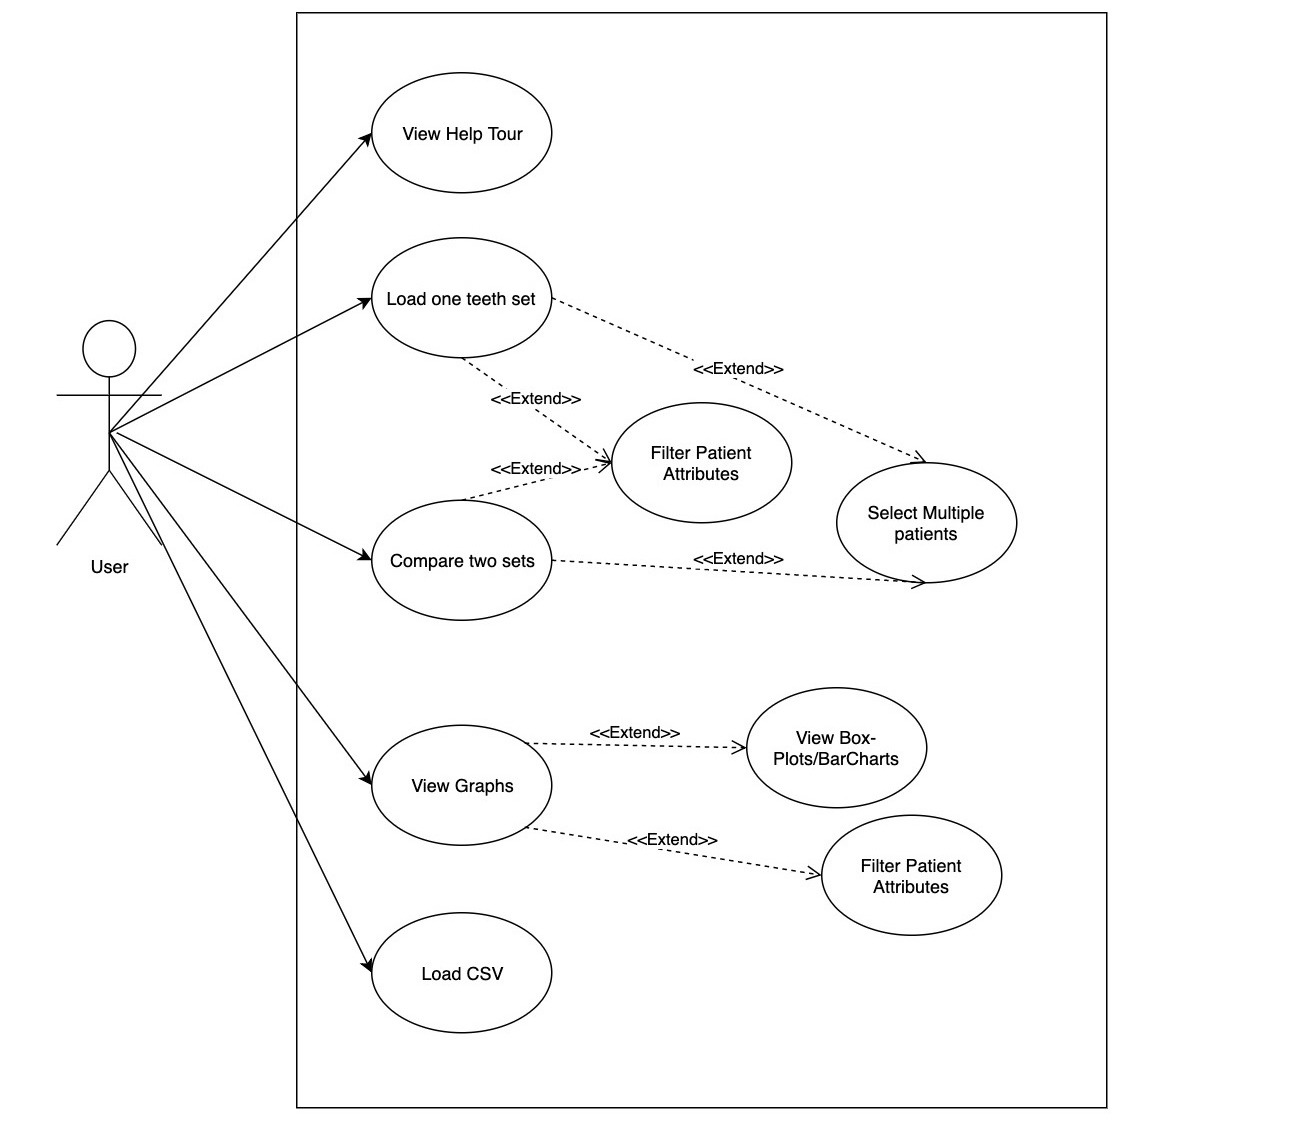
\includegraphics[width=120mm,scale=0.5]{usecase}
        \caption{Use Case Diagram}
        \label{fig:usecase}
        \end{center}
      \end{figure}

      We used Unity for our project, thus, we were inclined to adhere to Unity design standards. Unity design standards guide on how to structure the project, in aspects such as file structure and architecture. This is very important, as, for example, improper use of Resources folders will increase application startup time and the length of builds. Specifics for Unity design standards can be found on the Unity website: www.unity.com.
      One example that was particularly prominent for is, was the class all Game Objects must follow: all files that are game objects must inherit from the Unity root class, MonoBehaviour; these are slightly atypical such that they cannot be normally instantiated and thus not directly testable. \\
      \\
      Due to the use of Unity, we felt it was necessary to implement the ``Humble Object Design Pattern'' in our code, as it enabled us to take a test-driven development approach, which made development more agile and allowed us to make changes to code with ease when adapting to modifications in the client's requirements. Furthermore, due to Unity being commonly used for game development, achieving loose coupling is not a priority, as importance is placed on performance rather than maintainability, thus the decision to implement ``Humble Object Design Pattern'' was to also achieve loose coupling, high cohesion and SOLID code. \\
      \\
      We centred the design of our application around performance. As this is a live 3D rendering program, we took every step to ensure our program uses the least amount of system resources while also running smooth and looking sharp. Naturally, compromises had to be made. From the start, we knew this would be one of the key areas of concern. When designing the teeth model using Blender, we tried to minimise the number of polygons used while also trying to maintain a crisp image. As the teeth model can be rotated 360 degrees with zoom functionality and the ability to open and close the jaws, we took careful consideration when adding light sources to the scene. As the light sources are static and the teeth model is dynamic, shadows will be formed. By strategically placing the light sources and setting their intensity, we were able to get good lighting, reduce shadows while having only a few light sources, thus improving performance again. Adhering to these good Unity design standards, our application averages over 60fps, which is an industry standard.

      Below is an architecture diagram which shows how the Unity Engine interacts with the application that we have made. The ``Core Engine'' and ``Scene Manager'' interact with one another. The ``Scene Manager'' controls what scene is displayed to the user and as you can see, there are two types of scenes: Data Controller and Graph Controller. Data Controller is where the tutorial and all the actions that are related to the teeth model are situated, whereas Graph Controller is where all actions related to any type of graphs are located. This shows our use of the Model-View-Controller pattern, which provides many benefits to our codebase, one being the ability to cleanly test our logic classes, and the separation also allowing us to effectively pinpoint errors, and swiftly correct them as we progressed.\\


      \begin{figure}[H]
        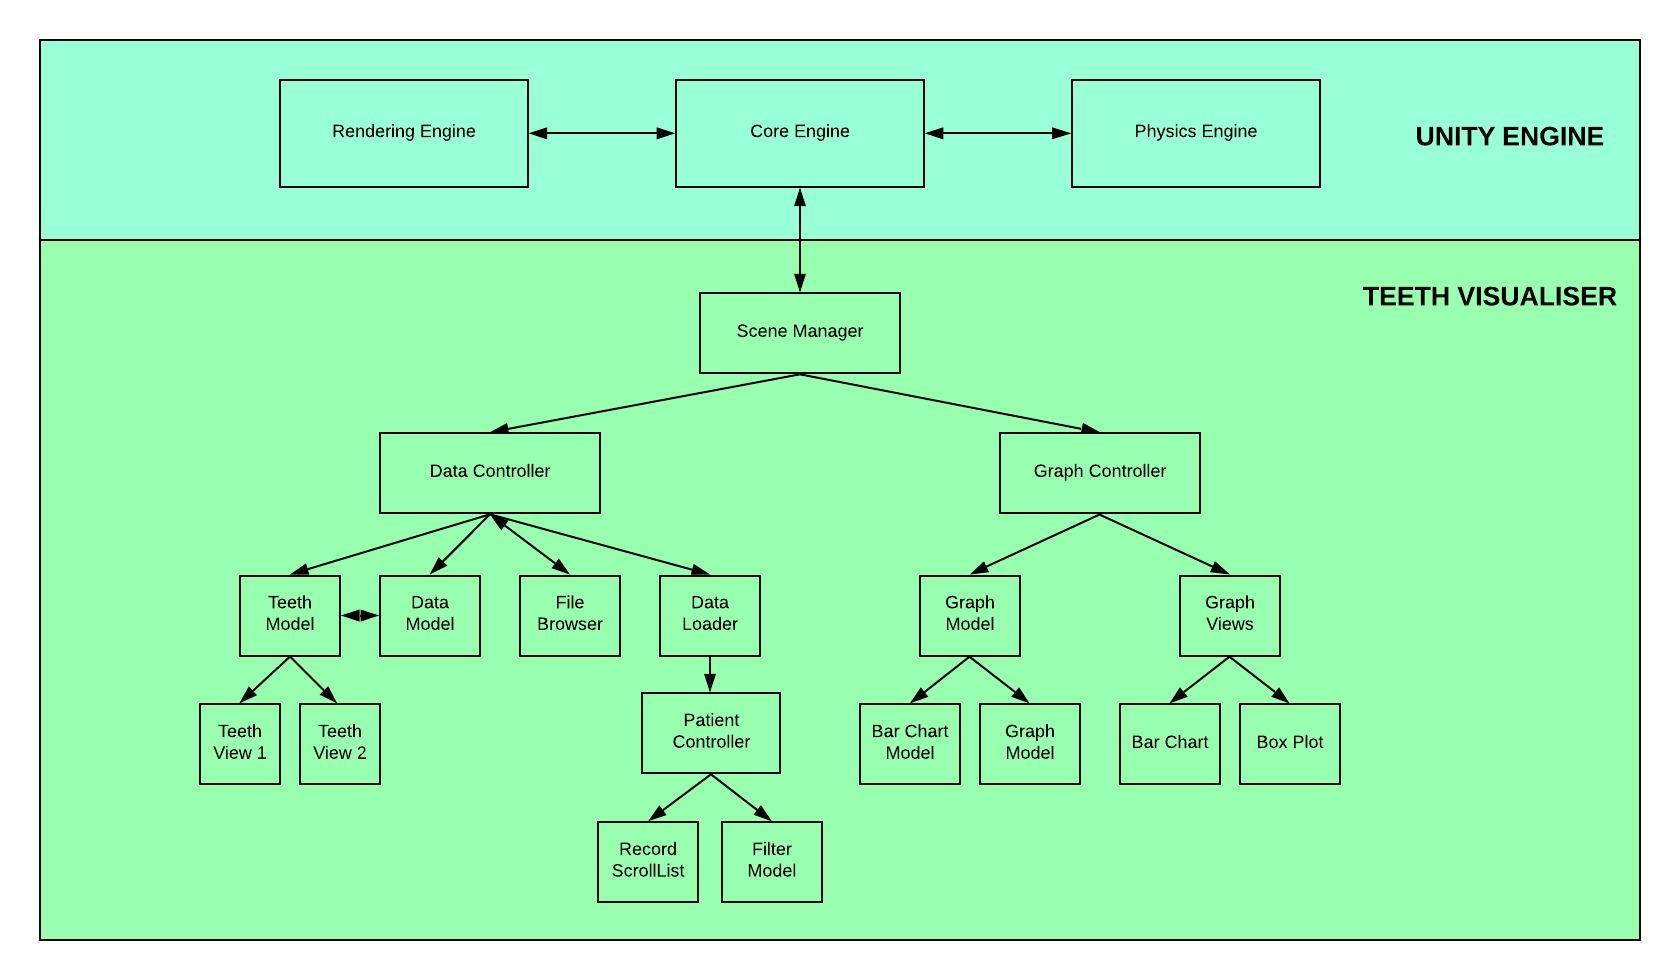
\includegraphics[width=\linewidth]{architecture}
        \caption{Architecture Diagram}
        \label{fig:architecture}
      \end{figure}

      \begin{figure}[H]
        \begin{center}
        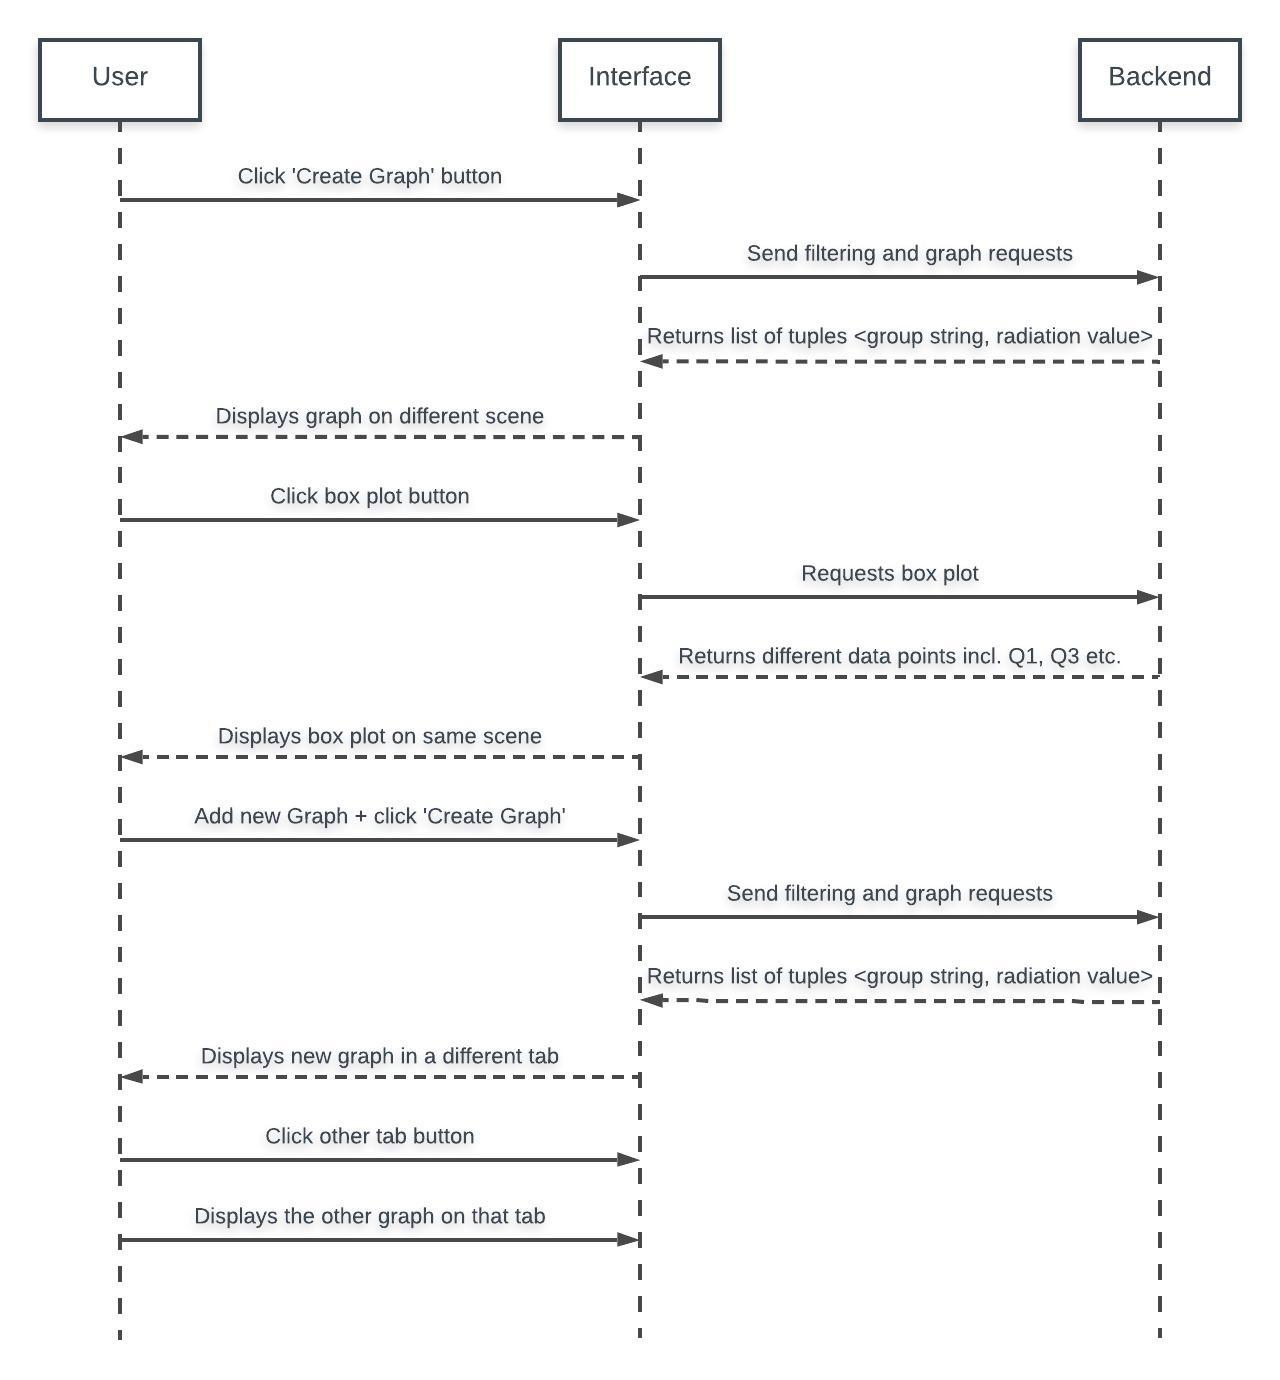
\includegraphics[width=100mm,scale=0.5]{graphsequence}
        \caption{Graph Sequence Diagram}
        \label{fig:graphsequence}
        \end{center}
      \end{figure}

  Figure 3 displays a sequence diagram describing the functionality of the ``Graphs'' feature of the application.

  \begin{figure}[H]
    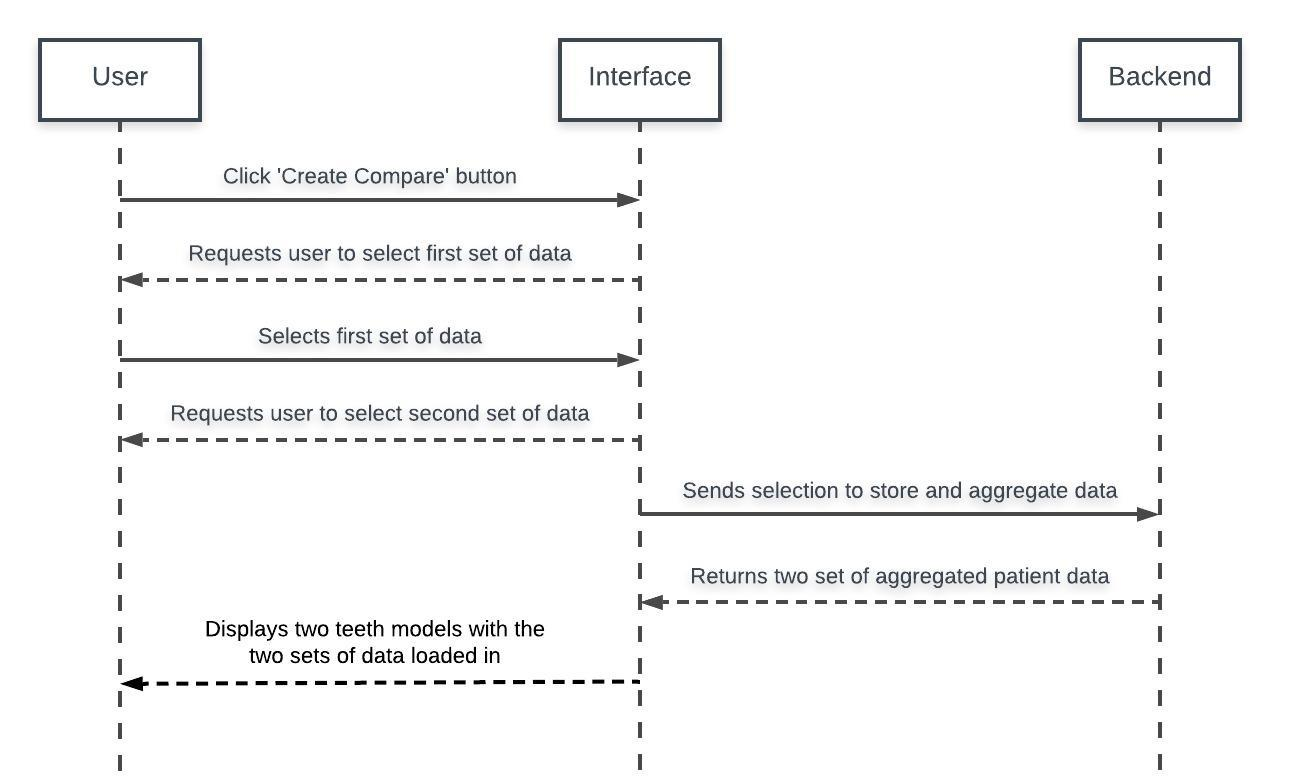
\includegraphics[width=\linewidth]{comparesequence}
    \caption{Compare Feature Sequence Diagram}
    \label{fig:comparesequence}
  \end{figure}


  \pagebreak
  \section*{Testing}
  % How you approached Testing
  % Explain testing tools employed
  % How software was sufficiently tested and where tests can be found
  The possibility of changes in requirements and giving the client early opportunities to see the software were two main reasons why we adopted the agile approach, resulting in using agile testing practices. \\
  \\
  From the beginning, we embraced the extreme programming practice, $'$Test first development$'$. We decided that it was more effective for each team member to be responsible for the testing of the user story that was assigned to themselves for each sprint, rather than creating a development team and a testing team. \\
  \\
  Thus, our main testing approach was ``Test Driven Development'' and the ``Humble Object Pattern'' using Unity's own test framework known as Unity Test Tools which includes: Unity Test Runner, a tool which integrates the NUnit library into Unity, allowing developers to perform unit testing; Integration Tests Runner, a tool which aids developers with integration testing. Also, acceptance testing was used alongside a screen recording $($Table can be found in ``Appendix''$)$ for UI testing as automated UI testing tools were very limited as Unity is a game development platform and is frequently used to develop games, thus importance is placed on the presentation of the game, which is difficult to create automated tests for. Moreover, we created a new class which provided mock data for testing, as that would remove the dependency on the CSV parser to be functional and also isolates the behaviour of the patients data and complexity of the class to simulate the behaviour. \\
  \\
  The ``Humble Object Pattern'' is when you extract all the logic from a component into a separate object and this approach was used because GUI objects, as mentioned before, are difficult to test efficiently for many reasons, including the need to use asynchronous tests due to Unity UI. This was an approach that made Unit testing possible and helped ensure us and the client that our code has been sufficiently tested .\\
  \\
  NUnit test scripts can be found in the ``Assets $\,\to\,$ Tests'' folder - please see the figure 5 as evidence of the 132 Unit Tests passing.\\
  \\
  Furthermore, to make sure the client was happy with the progress and the product, we regularly checked the application against the requirements and also set up meetings with the client to make sure that features were implemented correctly to the clients' satisfaction.

    \begin{figure}[H]
      \begin{center}
        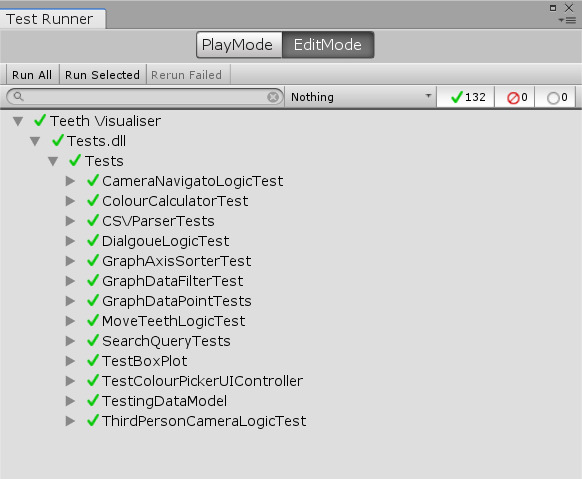
\includegraphics[width=100mm,scale=0.5]{test}
        \caption{Evidence of 132 Unit Tests Passing}
      \label{fig:test}
      \end{center}
    \end{figure}

  \section*{Team Organisation}
  The team was initially divided into 2 sub-groups; front-end and back-end teams.  The front-end team consisted of Logi, Awad,  and Aakash. The back-end team consisted of Michael, Haroon, Luca and Abs. Due to the nature of the project and the agile approach that we have taken, all team members started working on the front and back end tasks simultaneously. Some members were assigned additional roles, Haroon being the team leader, Logi the GitHub Master, Luca the team representative and Slack Master, Awad and Abs were responsible for recording the meetings on Team Feedback . We used the agile methodology with a sprint every week and a Kanban Board to track our progress. For testing, we took a test-driven approach with every member testing as the project progresses.  From weeks 1 to 3, Logi and Kim-Anh worked on the teeth model. Aakash and Awad worked on the UI and the rest of the team worked on the backend. From week 4 onwards, Logi focused on the front and back end of the model colour with radiation. Aakash, Abs and Kim-Anh worked on the Graph implementation. Luca worked on the camera. Haroon worked on the data parser. Awad, Aakash and Michael worked on the UI with Michael also working on the backend architecture.
  \\
  \section*{Other Pertinent Information}
  Our team maintained important documentation such as a Risk register, a Gantt Chart, Acceptance testing form and other documents on our google drive. Link to the google drive is below.\\

  Link: \url{https://drive.google.com/drive/folders/1rU73zZ3FfNZOgyy0Eulj4GX_ffmgQVlr} \\
  \\
  The Risk Register was used to document risks, and actions to manage each risk. It was accompanied by a Risk Assessment Matrix to help us classify each risk. We also had a Risk Management document. Our Acceptance testing form had the procedure number, the name of the input/procedure, the expected result/output, a tick box for whether the test passed and a timestamp for when the procedure is done in our screencast. This acceptance testing form was crucial in our testing as in Unity you can't test the User Interface components. \\
  \\
  Due to the nature of this project involving computer graphics and none of our team members having done any graphics related work beforehand, there was a steep learning curve for all members of the team. We spent the first weeks researching on which graphics engine to use. After our first client meeting with Dr Sassoon the requirements became much clearer, so we decided to use Unity. The team spent another 2 weeks learning Unity.  We had a few hiccups that we were able to overcome like some of the team members found their scripts and animations to be missing every time they pulled from remote, thanks to our Git Master Logi, we were able to trace the problem back to the gitignore file in the repo having a  .meta tag in it. With the resilience and determination of the team, we were able to overcome many such hiccups that arose due to Unity being a foreign object to us at first but now is like second nature. \\
  \\
  Major changes in the requirements occurred over the course of the project, such as the ``Compare'' feature which was not specified in the requirements beforehand and also the ability to visualise the data sets as box plots, which was required by the client later on in the project. Furthermore, it was discovered that the client also wanted to pick their own colours for the heatmap which would be applied to each tooth depending on their values within the range specified. All modifications in the requirements were taken aboard and implemented. \\
  \\
  \underline{Extendability} \\
  \\
  During the development of the project, we took into consideration the possibility of adding new features as the requirements of the client changed over time. These features include:

  \begin{itemize}
    \item The ability to have a four-way split screen
    \item Split screen graphs
    \item Adding more types of graphs and more graph features, such as overlaying different graphs
    \item More advanced tutorial tour with interactive features
    \item Improved 3D teeth model
    \item More sleek UI
    \item More advanced file management system
    \item Using machine learning to aid in pattern recognition in data sets provided
  \end{itemize}

  \section*{Appendix}
    \begin{center}
    \begin{tabular}{ | c | c | c | c | c |}
      \hline
      \thead{Procedure \\ No.} & \thead{Input$/$Procedure} & \thead{Expected Result$/$Output} & \thead{Passed} & \thead{Video \\ Time} \\
      \hline
      1 & Opening desktop application & \makecell{All teeth models and buttons \\ are displayed on the screen} & \checkmark & 2:16 \\
      \hline
      2 & \makecell{Displaying filtered list \\ of patients} & \makecell{---} & \checkmark & - \\
      \hline
      2.1 & \makecell{Clicking left sidebar button \\ \textit{$($SidebarButton.cs$)$}} & \makecell{
        Panel slides from the left and \\ is visible to user. Contains \\ dropdown lists and sliders.
        } & \checkmark & 3:06\\
      \hline
      2.2 & \makecell{Clicking dropdown buttons \\ \textit{$($Dropdown.cs$)$}} & \makecell{Dropdown expands to show \\ list of toggles} & \checkmark & 6:02\\
      \hline
      2.2.1 & \makecell{Clicking a toggle that is not \\ ``All'' \\ \textit{$($Dropdown.cs$)$}} & \makecell{``All'' toggle automatically is \\ turned off} & \checkmark & 6:25\\
      \hline
      2.2.2 & \makecell{Unselecting all toggles \\ \textit{$($Dropdown.cs$)$}} & \makecell{Application will not allow the \\ unselection of all toggles} & \checkmark & N/A\\
      \hline
      2.3 & \makecell{Modify the age min-max \\ slider \\ \textit{$($MinMaxSlider.cs$)$}} & \makecell{Numbers on top of the slider \\ changes dependent on the \\ positions of the 2 buttons.} & \checkmark & 6:36\\
      \hline
      2.4 & \makecell{Click ``Filter'' button \\ \textit{$($UserInput.cs$)$}} & \makecell{List of patients $($results$)$ are \\ displayed in the panel \\ underneath the filter \\components and are within \\the age range specified.} & \checkmark & 6:44\\
      \hline
      3 & \makecell{Click ``Reset'' button on the filter \\ panel \\ \textit{$($Dropdown.cs$)$}} & \makecell{All filters and lists of patients are \\ resetted to default positions} & \checkmark & 7:48\\
      \hline
      4 & \makecell{Click ``Select All'' \\ \textit{$($RecordScrollList.cs$)$}}  & \makecell{All instances of the displayed \\ patients are selected} & \checkmark & 8:29\\
      \hline
      4.1 & \makecell{Click ``Select All'' again \\ \textit{$($RecordScrollList.cs$)$}} & \makecell{All instances of the displayed \\ patients are unselected} & \checkmark & 8:33\\
      \hline
      5 & \makecell{Loading one patient onto teeth \\ model \\ \textit{$($Search Query.cs, RecordScrollList.cs} \\ \textit{UserInput.cs$)$}} & \makecell{---} & \checkmark & -\\
      \hline
      5.1 & \makecell{Click ``Load'' button without \\ selecting a patient/s} & \makecell{Displays error message} & \checkmark & N/A\\
      \hline
      5.2 & \makecell{Select one patient from the list \\ \textit{$($DisplayButton.cs$)$}} & \makecell{Whole row is highlighted} & \checkmark & 3:52\\
      \hline
      5.3 & \makecell{Click ``Load'' button} & \makecell{Panel collapses and teeth model \\ is visible } & \checkmark & 3:56\\
      \hline
    \end{tabular}
  \end{center}

\begin{center}
\begin{tabular}{ | c | c | c | c | c |}
  \hline
  \thead{Procedure \\ No.} & \thead{Input$/$Procedure} & \thead{Expected Result$/$Output} & \thead{Passed} & \thead{Video \\ Time} \\
  \hline
  5.4 & \makecell{Hover over different teeth on \\ teeth model \\ \textit{$($TeethScriptAssigner.cs$)$} \\ \textit{$($TeethDisplayPanel.cs$)$}} & \makecell{Radiation values are displayed on \\ the top left and changes depending \\ on where the mouse pointer is at} & \checkmark & 6:02\\
  \hline
  6 & \makecell{Clicking ``Reset'' button \\ \textit{$($ResetTeeth.cs$)$}} & \makecell{When hovering over the teeth, no \\ radiation values should appear on \\ screen, indicating data has been \\ removed from the model} & \checkmark & - \\
  \hline
  7 & \makecell{Loading many patients onto one \\ teeth model +  aggregate \\ function \textit{$($DataModel.cs$)$}} & \makecell{---} & --- & --- \\
  \hline
  7.1 & \makecell{Select the same patient from \\ Procedure 5 and another random \\ patient} & \makecell{Two rows are highlighted} & \checkmark & 7:10 \\
  \hline
  7.2 & \makecell{Click ``Load'' button} & \makecell{Panel collapses and teeth model is \\ visible} & \checkmark & 7:12 \\
  \hline
  7.3 & \makecell{Hover over different teeth on \\ teeth model} & \makecell{Should observe an increase in \\ radiation values from Procedure 5 \\ when hovering over the teeth.} & \checkmark & 4:10 \\
  \hline
  8 & \makecell{Comparing 2 sets of data using \\ teeth model \\ \textit{$($ComparePatients.cs$)$}} & \makecell{---} & --- & --- \\
  \hline
  8.1 & \makecell{Click ``Compare'' button} & \makecell{Button displays ``Select First Set''} & \checkmark & 8:09 \\
  \hline
  8.2 & \makecell{Select 1 or more patients from \\ the list and click Select First \\ Set button} & \makecell{Button displays ``Select Second Set''} & \checkmark & 8:19 \\
  \hline
  8.3 & \makecell{Select 1 or more patients from \\ the list and click Select Second \\ Set button TeethScriptAssigner} & \makecell{Behind the filter panel, two teeth \\ models are displayed} & \checkmark & 8:40 \\
  \hline
  9 & \makecell{Camera Lock + Cube Navigation \\ \textit{$($ThirdPersonCamera.cs} \\ \textit{CameraNavigator.cs$)$}} & \makecell{---} & --- & --- \\
  \hline
  9.1 & \makecell{Default setting is camera is \\ locked + drag the navigation \\ cube around} & \makecell{Both teeth are moving \\ simultaneously in the same \\ direction} & \checkmark & 8:49 \\
  \hline
  9.2 & \makecell{Unlock camera lock} & \makecell{Two navigation cubes are displayed. \\ One for each teeth model so they \\ are able to move independently of \\ one another.} & \checkmark & 9:04 \\
  \hline
  10 & \makecell{Move zoom slider back and forth \\ \textit{$($ThirdPersonCamera$)$}} & \makecell{Camera can zoom in and out of \\ teeth model/s} & \checkmark & 2:45 \\
  \hline
\end{tabular}
\end{center}

\begin{center}
\begin{tabular}{ | c | c | c | c | c |}
  \hline
  \thead{Procedure \\ No.} & \thead{Input$/$Procedure} & \thead{Expected Result$/$Output} & \thead{Passed} & \thead{Video \\ Time}\\
  \hline
  11 & \makecell{Display Patient Details \\ \textit{$($LoadPatient.cs$)$}} & \makecell{---} & --- & --- \\
  \hline
  11.1 & \makecell{Click on ``Patient Details'' at the \\ bottom left} & \makecell{Shows aggregated details of all \\ patients in first set} & \checkmark & 10:20 \\
  \hline
  11.2 & \makecell{Click on ``Patient Details'' at the \\ bottom right} & \makecell{Shows aggregated details of all \\ patients in second set} & \checkmark & 10:18 \\
  \hline
  12 & \makecell{Visualise radiation using colours \\ \textit{$($ColourCalculator, ColourPickerUI} \\ \textit{ColourPickerUIController, ColourSelect$)$}} & \makecell{---} & --- & --- \\
  \hline
  12.1 & \makecell{Open ``Colour Picker'' panel by \\ clicking the button with an \\ arrow on the right hand side} & \makecell{Two input fields, seven colours, 4 \\ buttons and information on the min \\ and max radiation of each set of \\ teeth are displayed} & \checkmark & 5:02 \\
  \hline
  12.2 & \makecell{Insert non-numeric characters \\ inside the input field and click \\ ``Apply''} & \makecell{Panel collapses and ``Invalid input!'' \\ is displayed on the screen.} & \checkmark & N/A \\
  \hline
  12.3 & \makecell{No patients are loaded onto the \\ teeth model and you try to apply \\ colours to the model} & \makecell{Panel collapses and ``No patients \\ selected!'' is displayed on the screen} & \checkmark & N/A \\
  \hline
  12.4 & \makecell{One patient is loaded in and try \\ to apply colours to second model} & \makecell{Error message displayed} & --- & --- \\
  \hline
  12.5 & \makecell{Insert a number in both input \\ fields and click ``Apply''} & \makecell{Panel collapses and ``Invalid \\ range!'' is displayed on the screen} & --- & N/A \\
  \hline
  12.6 & \makecell{Input in ``From'' field is larger \\ then input in ``To'' field} & \makecell{Button displays ``Select First Set''} & \checkmark & N/A \\
  \hline
  12.7 & \makecell{Input in ``From'' field is less then \\ input in ``To'' field, 2 colours are \\ selected and click ``Apply'' button} & \makecell{Colour within the gradient between \\ the two colours chosen are applied \\ to the teeth. On ``Colour Picker'' \\ panel, gradient bar and the \\radiation range is displayed} & \checkmark & 5:10 \\
  \hline
  12.8 & \makecell{Input in ``From'' field is less then \\ input in ``To'' field, 2 colours are \\ selected and click ``Apply Second \\ Set'' button} & \makecell{Colour within the gradient between \\ the two colours chosen are applied \\ to the second set of teeth. On \\ ``Colour Picker'' panel, gradient bar \\ and the radiation range is displayed} & \checkmark & 9:56 \\
  \hline
  12.9.1 & \makecell{Click ``Reset colour map A''} & \makecell{Gradient bar on panel and colour \\ on first teeth model disappears} & \checkmark & 5:34  \\
  \hline
  12.9.2 & \makecell{Click ``Reset colour map B''} & \makecell{Gradient bar on panel and colour \\ on second teeth model disappears} & \checkmark & N/A \\
  \hline
  13 & \makecell{Add CSV file \\ \textit{$($CSVParser.cs$)$}} & \makecell{---} & --- & --- \\
  \hline
\end{tabular}
\end{center}

\begin{center}
\begin{tabular}{ | c | c | c | c | c | }
  \hline
  \thead{Procedure \\ No.} & \thead{Input$/$Procedure} & \thead{Expected Result$/$Output} & \thead{Passed} & \thead{Video \\ Time} \\
  \hline
  13.1 & \makecell{Click ``Add CSV File'' on navbar} & \makecell{New window appears which is the \\ file manager.} & \checkmark & 3:18 \\
  \hline
  13.2 & \makecell{Click on a non-CSV file} & \makecell{Unable to select file} & \checkmark & 3:24 \\
  \hline
  13.3 & \makecell{Select a CSV file and click \\ upload button} & \makecell{---} & \checkmark & 3:37 \\
  \hline
  13.4 & \makecell{Click X on file manager \\ window} & \makecell{Window disappears} & \checkmark & N/A \\
  \hline
  14 & \makecell{Creating graphs \\ \textit{$($Graph, GraphData,} \\ \textit{ GraphDataPoint,} \\ \textit{ BarChartVisual,} \\ \textit{BoxPlotVisual, SceneTransition$)$}} & \makecell{---} & --- & --- \\
  \hline
  14.1 & \makecell{Click ``Graphs'' on the navbar} & Filter panel should appear beneath & \checkmark & 11:03 \\
  \hline
  14.2 & \makecell{Under ``X Axis'', select ``Age'' \\ from the dropdown} & \makecell{Input field should appear \\ on the panel} & \checkmark & 11:14 \\
  \hline
  14.3.1 & \makecell{Enter non-numeric characters in \\ input field} & \makecell{Unable to enter non-numeric \\ characters} & \checkmark & N/A \\
  \hline
  14.3.2 & \makecell{Enter a number $\leq$ 0} & \makecell{Displays error message} &  &  N/A \\
  \hline
  14.4 & \makecell{Click ``Create Graph'' when \\ ``Age'' is selected for the x axis \\ and the input field is empty} & \makecell{Displays error message} & \checkmark  & N/A  \\
  \hline
  14.5 & \makecell{Under ``X Axis'', select any \\ option bar ``Age'' from the \\ dropdown} & \makecell{Input field disappears} & \checkmark & N/A \\
  \hline
  14.6 & \makecell{Click ``Graphs'' or ``Cancel'' } & \makecell{Filter panel closes} & \checkmark & N/A \\
  \hline
  14.7 & \makecell{Select ``Nodal'' as the X axis and \\ filter the patients to show only \\ N0, N1 and N2. Then click \\ ``Create Graph''} & \makecell{New scene appears, initially \\ showing a bar chart that only \\ consists of average radiation values \\ for patients that have N0, N1 or N2. \\ Y axis and bars have scaled \\ correctly} & \checkmark & N/A \\
  \hline
  14.8 & \makecell{Click on ``BoxPlotButton''} & \makecell{Bar chart is converted to a box plot \\ which can also include outliers} & \checkmark & 11:25 \\
  \hline
  15 & \makecell{If graph has many data points, \\ graph is scrollable. $($X Axis \\ variable is Patient$)$} & \makecell{Can scroll with your trackpad or \\ using the the scrollbar} & \checkmark & N/A \\
  \hline
  15.1.1 & \makecell{Press + button near the tabs \\ Click ``Create Graph''} & \makecell{Filter panel is displayed \\
New tab and graph are displayed on \\ a different tab} & \checkmark & N/A \\
  \hline

\end{tabular}
\end{center}

\begin{center}
\begin{tabular}{ | c | c | c | c | c |}
  \hline
  \thead{Procedure \\ No.} & \thead{Input$/$Procedure} & \thead{Expected Result$/$Output} & \thead{Passed} & \thead{Video \\ Time} \\
  \hline
  15.1.2 & \makecell{Click ``New Graph'' button \\Click ``Create Graph''} & \makecell{Filter panel is displayed \\ New tab and graph are displayed on \\ a different tab} & \checkmark & N/A \\
  \hline
  15.2 & \makecell{Click ``New Graph'' button. \\ Click + to add a tab} & \makecell{Duplicate graph is created} & \checkmark & 11:50 \\
  \hline
  15.3 & \makecell{Click on previous opened tab} & \makecell{Transitions into the old graph} & \checkmark & 12:09 \\
  \hline
  15.4 & \makecell{Open 4 new tabs and \\ click ``New Graph'' then \\ ``Create Graph''} & \makecell{Last tab is replaced with new graph} & \checkmark & N/A \\
  \hline
  15.5 & \makecell{Hovering over bars in bar graph} & \makecell{Tooltip displayed over the bar \\ showing the exact radiation value.} & \checkmark & 11:58 \\
  \hline
  15.6 & \makecell{Click X on the top-right corner} & \makecell{Home scene is displayed, where \\ you can see the teeth model} & \checkmark & 12:35 \\
  \hline
  16 & \makecell{Tutorial Tour \\ \textit{Dialogue, DialogueManager, } \\ \textit{DialogueTrigger}} & \makecell{---} & --- & 12:44 \\
  \hline
  16.1 & \makecell{Click ``Help'' on the navbar} & \makecell{A panel should appear with letters \\ appearing one by one} & -\checkmark & 13:09 \\
  \hline
  16.2 & \makecell{Click ``Continue''} & \makecell{New text is displayed onto the panel \\ and should be invoking different \\ actions across the application} & \checkmark & 14:30 \\
  \hline
  16.3 & \makecell{End of tutorial} & \makecell{Should consist of 23 steps} & \checkmark & 14:43 \\
  \hline
\end{tabular}
\end{center}
\pagebreak
\section*{References}
  \begin{itemize}
    \item \textbf{Max-Min Slider} \\
    \url{https://github.com/brogan89/MinMaxSlider}
    \item \textbf{Graph Icons} \\
    \url{https://icons8.com/icon/15/bar-chart} Bar Chart icon by Icons8 \\
    Box Plot Graph - Designed by Freepik from Flaticon \\
    \url{https://icons8.com/icon/1510/multiply} Multiply icon by Icons8
    \item \textbf{Basic Graph Structure} \\
    \url{https://unitycodemonkey.com/video.php?v=CmU5-v-v1Qo}
    \item \textbf{File Manager} \\
    \url{https://github.com/GracesGames/SimpleFileBrowser}
    \item \textbf{Teeth Model} \\
    \url{https://www.blender.org/}
    \item \textbf{The Whole Application} \\
    \url{hhttps://unity.com/}
  \end{itemize}
\end{document}
